\section{Data Analysis}




Now we aim to investigate how the wishlist are being used by online shoppers and its market implications. We aim to show user shopping preference in different regions and different time periods. Besides, we also analyze different user shopping tendencies in holidays and normal days.
\subsection{basic statistics}
We use our data in different ways. The very first step is to conduct fundamental measurements on the dataset. We wish to help people understand usage of wish lists and to what extent do the users expose their personal information in Amazon. 

For all 967,603 users collected in the first step of data collection, there are totally 2,121,173 wish lists recorded, which indicates that each user has 2.2 wish lists in average. Table~\ref{tb:stat} illustrates personal information exposure in user list profiles. We found that a considerable number of users put their birthday and location information in their list profiles. Furthermore, most of the people who have a list-description have exposed their birthday and address information. Our findings agree with \cite{frankowski2006you}, which states that users tend to expose their personal information in open websites. 

\begin{table}[!htbp]
\centering
\caption{Personal Information in User Profile}
\label{tb:stat}
\begin{adjustbox}{max width=.5\textwidth}
\begin{tabular}{lll}
Personal Info & User Number & Percentage \\
Birthday & 280,328 & 29.0\% \\
Location & 221,298 & 22.9\% \\
Birthday \& Location & 150,004 & 15.5\% \\
List-description & 104,846 & 10.8\% \\
List-description \& Birthday & 94,284 & 9.7\% \\
List-description \& Location & 59,731 & 6.2\% 
\end{tabular}
\end{adjustbox}
\end{table}




\begin{figure*}[!htb]
\minipage{0.32\textwidth}
  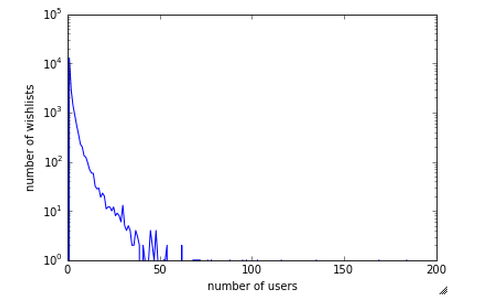
\includegraphics[width=\linewidth]{avglist.png}
  \caption{Number of lists the users have}\label{avglist}
\endminipage\hfill
\minipage{0.32\textwidth}
  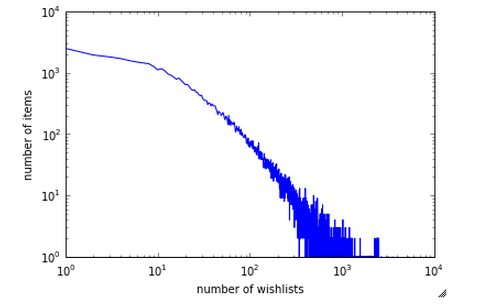
\includegraphics[width=\linewidth]{avgitem.png}
  \caption{Number of items the lists have}\label{avgitem}
\endminipage\hfill
\minipage{0.32\textwidth}%
  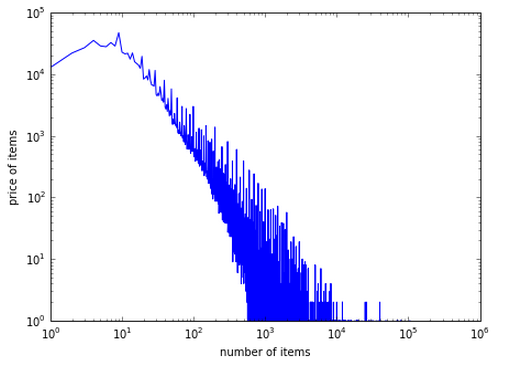
\includegraphics[width=\linewidth]{avgprice.png}
  \caption{Item Price}\label{avgprice}
\endminipage
\end{figure*}

First we 

Then we present the statistics of wishlist usage. As we did not collect the wishlist items of all the users, we analyze only the 20099 users that are completely collected. Among the 20,099 users, we recorded 48,848 full wish lists, which means not only are the wishlists names and URLs are recorded, but also the items in the wishlists. The average number of wishlists a user has is 2.43, which is a little higher than that of the whole dataset. We believe the little gap is reasonable because the users who have filled the list-descriptions tend to use the feature of wishlists more so they are more prone to input personal information and products in their profiles. We further explore the distribution of the number of wish list a user has, which is shown in Figure~\ref{avglist}. Similarly, we show the distribution of the number of wish list a user has in Figure~\ref{avgitem}. Another thing we are interested in is the price of the items. The average price of all the items 47.16 US dollars. The distribution of the prices are shown in Figure~\ref{avgprice}. 

\begin{table}[!htbp]
\centering
\caption{Distribution}
\label{tb:stat2}
\begin{adjustbox}{max width=.5\textwidth}
\begin{tabular}{llllll}
Distribution & Mean & Max & SD & $\gamma$ & $\kappa$ \\
Wishlist in Profile & 2.43 & 184 &? &? &? \\
Items in Wishlist & 68 & 5,238 & ? & ? & ?\\
Item Price & 47.16 & ? & ? & ? & ? \\
\end{tabular}
\end{adjustbox}
\end{table}

We have analyzed the basic usage of wishlists and item price. Now we show user shopping preference and pattern in general as well as in different regions. 

\subsection{User preference in different regions}

\begin{table}[!htbp]
\centering
\caption{EAST COAST USER PREFERENCE}
\label{tb:east}
\begin{adjustbox}{max width=.5\textwidth}
\begin{tabular}{lllll}
Rank & Item Type          & Number of Items & Percentage of Items & Average Price(\$) \\
1 & Books & 1053832 & 38.79\% & \$14.95 \\
2 & Movies \& TV & 315661 & 11.62\% & \$19.93 \\
3 & CDs \& Vinyl & 200312 & 7.37\% & \$11.62 \\
4 & Buy a Kindle & 182089 & 6.70\% & \$9.00 \\
5 & Toys \& Games & 151982 & 5.59\% & \$33.98 \\
6 & default & 138133 & 5.08\% & \$28.02 \\
7 & Amazon Fashion & 88116 & 3.24\% & \$34.83 \\
8 & Video Games & 67627 & 2.49\% & \$41.75 \\
9 & Sports \& Outdoors & 61475 & 2.26\% & \$44.30 \\
10 & Kitchen \& Dining & 58983 & 2.17\% & \$39.67 \\
11 & Home \& Kitchen & 52739 & 1.94\% & \$47.24 \\
12 & Home Improvement & 39401 & 1.45\% & \$54.85 \\
13 & All Electronics & 35347 & 1.30\% & \$81.30 \\
14 & Health \& Personal Care & 25923 & 0.95\% & \$30.75 \\
15 & All Beauty & 22925 & 0.84\% & \$20.48 \\
16 & Computers & 22920 & 0.84\% & \$98.60 \\
17 & Camera \& Photo & 22894 & 0.84\% & \$145.10 \\
18 & Digital Music & 19986 & 0.74\% & \$7.53 \\
19 & Patio, Lawn \& Garden & 17869 & 0.66\% & \$56.52 \\
20 & Grocery \& Gourmet Food & 16999 & 0.63\% & \$18.58 \\
\end{tabular}
\end{adjustbox}
\end{table}

We analyze the user preference in different regions, which are -- east coast, west coast, and middle of the US according to Wikipedia \cite{east}\cite{west}. It is natural to consider that people may have different shopping preference in different regions. We quantitatively show the differences in this section as well as presenting interesting observations. The average price of east coast, west coast, and middle of US is \$25.69, \$27.33 and \$24.87 accordingly. As the price in Amazon will not be different for users from different regions, our result indicates that the price sensitivity is highest in middle area of the US, and is lowest in the west coast area. It agrees with the common knowledge -- the average income in coastal area is higher than the middle area, and the west coast is higher than the east coast. 

We further look into the detailed The top 20 preferences for people from east coast is shown in Table~\ref{tb:east}. The top 20 preferences for people from west coast is shown in Table~\ref{tb:west} and the top 20 preferences for people from middle of the US is shown in Table~\ref{tb:mid}

\begin{table}[!htbp]
\centering
\caption{EAST COAST USER PREFERENCE}
\label{tb:east}
\begin{adjustbox}{max width=.5\textwidth}
\begin{tabular}{lllll}
Rank & Item Type          & Number of Items & Percentage of Items & Average Price(\$) \\
1 & Books & 210205 & 41.44\% & \$6.19 \\
2 & Movies \& TV & 63648 & 12.55\% & \$17.11 \\
3 & CDs \& Vinyl & 46726 & 9.21\% & \$9.75 \\
4 & Buy a Kindle & 25859 & 5.10\% & \$9.77 \\
5 & Toys \& Games & 25542 & 5.04\% & \$41.73 \\
6 & Sports \& Outdoors & 15619 & 3.08\% & \$48.73 \\
7 & Video Games & 14819 & 2.92\% & \$31.01 \\
8 & Amazon Fashion & 11379 & 2.24\% & \$45.26 \\
9 & All Electronics & 9054 & 1.79\% & \$123.91 \\
10 & Home Improvement & 8929 & 1.76\% & \$60.18 \\
11 & Kitchen \& Dining & 8209 & 1.62\% & \$53.59 \\
12 & Home \& Kitchen & 6702 & 1.32\% & \$58.87 \\
13 & Camera \& Photo & 5647 & 1.11\% & \$314.25 \\
14 & Computers & 5516 & 1.09\% & \$119.79 \\
15 & Health \& Personal Care & 4302 & 0.85\% & \$48.56 \\
16 & Digital Music & 3776 & 0.74\% & \$0.00 \\
17 & Patio, Lawn \& Garden & 3642 & 0.72\% & \$88.11 \\
18 & Automotive & 3478 & 0.69\% & \$62.53 \\
19 & Musical Instruments & 3157 & 0.62\% & \$154.15 \\
20 & Cell Phones \& Accessories & 2867 & 0.57\% & \$37.65 \\
\end{tabular}
\end{adjustbox}
\end{table}

\begin{table}[!htbp]
\centering
\caption{WEST COAST USER PREFERENCE}
\label{tb:west}
\begin{adjustbox}{max width=.5\textwidth}
\begin{tabular}{lllll}
Rank & Item Type          & Number of Items & Percentage of Items & Average Price(\$) \\
1 & Books & 145939 & 41.99\% & \$6.10 \\
2 & Movies \& TV & 46266 & 13.31\% & \$16.52 \\
3 & CDs \& Vinyl & 33981 & 9.78\% & \$8.85 \\
4 & Buy a Kindle & 18072 & 5.20\% & \$9.98 \\
5 & Toys \& Games & 16351 & 4.70\% & \$40.03 \\
6 & Sports \& Outdoors & 9191 & 2.64\% & \$57.02 \\
7 & Video Games & 8708 & 2.51\% & \$30.75 \\
8 & Amazon Fashion & 7223 & 2.08\% & \$85.60 \\
9 & Home Improvement & 7002 & 2.01\% & \$66.70 \\
10 & All Electronics & 6756 & 1.94\% & \$147.81 \\
11 & Kitchen \& Dining & 4905 & 1.41\% & \$51.04 \\
12 & Home \& Kitchen & 4448 & 1.28\% & \$71.36 \\
13 & Camera \& Photo & 4267 & 1.23\% & \$322.14 \\
14 & Computers & 3908 & 1.12\% & \$117.42 \\
15 & Digital Music & 2921 & 0.84\% & \$0.00 \\
16 & Health \& Personal Care & 2801 & 0.81\% & \$40.73 \\
17 & Automotive & 2383 & 0.69\% & \$63.70 \\
18 & Musical Instruments & 2022 & 0.58\% & \$128.10 \\
19 & Cell Phones \& Accessories & 1878 & 0.54\% & \$36.98 \\
20 & Patio, Lawn \& Garden & 1808 & 0.52\% & \$108.02 \\
\end{tabular}
\end{adjustbox}
\end{table}

\begin{table}[!htbp]
\centering
\caption{MIDDLE OF US USER PREFERENCE}
\label{tb:mid}
\begin{adjustbox}{max width=.5\textwidth}
\begin{tabular}{lllll}
Rank & Item Type          & Number of Items & Percentage of Items & Average Price(\$) \\
1 & Books & 362966 & 43.96\% & \$8.27 \\
2 & Movies \& TV & 112737 & 13.65\% & \$16.11 \\
3 & CDs \& Vinyl & 75685 & 9.17\% & \$9.19 \\
4 & Buy a Kindle & 43510 & 5.27\% & \$9.37 \\
5 & Toys \& Games & 42419 & 5.14\% & \$37.36 \\
6 & Video Games & 24587 & 2.98\% & \$29.93 \\
7 & Sports \& Outdoors & 20101 & 2.43\% & \$50.90 \\
8 & Amazon Fashion & 16635 & 2.01\% & \$76.39 \\
9 & Home Improvement & 12977 & 1.57\% & \$69.84 \\
10 & All Electronics & 12009 & 1.45\% & \$124.05 \\
11 & Kitchen \& Dining & 11292 & 1.37\% & \$45.95 \\
12 & Home \& Kitchen & 10321 & 1.25\% & \$59.15 \\
13 & Camera \& Photo & 7488 & 0.91\% & \$338.27 \\
14 & Computers & 6993 & 0.85\% & \$125.67 \\
15 & Digital Music & 6965 & 0.84\% & \$0.00 \\
16 & Health \& Personal Care & 5458 & 0.66\% & \$37.70 \\
17 & Automotive & 5021 & 0.61\% & \$66.18 \\
18 & Patio, Lawn \& Garden & 4666 & 0.57\% & \$101.79 \\
19 & Musical Instruments & 4245 & 0.51\% & \$151.28 \\
20 & Grocery \& Gourmet Food & 3915 & 0.47\% & \$18.99 \\
\end{tabular}
\end{adjustbox}
\end{table}

From the tables we have the following observations.

\begin{enumerate}
\item Books are dominating the wish lists in these areas with all over 40\% of the items being books.

\item There are more reading lovers in the middle area of the US. Although the price sensitivity is highest in the middle area, people there are more likely to accept higher price on books, given that the average price of books in the middle area is 33.6\% and 35.6\% higher than east and west coast correspondingly. 

\item Besides books, entertainment also plays an important roles. Movies\& TV and CDs \& Vinyl rank second and third in the wish lists. In fact, in all the 3 areas, the top categories are basically the same, which means that people from different regions are likely to buy similar types of products. 

\item There are still differences in user shopping preference. For example, people from west and middle are willing to pay much more in fashion (clothing, shoes, etc) than people from east (west -- \$85.6, middle -- \$76.4, east -- \$45.3). On the other hand, people from east are willing to pay more in Health \& Personal care (around 20\% higher in average price). Besides, people from coastal areas seem purchasing more electronics and computers than the middle area. Besides, People from west are more tolerable to high prices in Sports \& Outdoors products. 

\end{enumerate}
In conclusion, these information is valuable to companies to promote their products and advertisers to find the price preferences for different users. 

\subsection{Holidays}
In this section we measure how the items are added in the wish lists during holidays and normal days. As there are many unofficial or regional holidays, in our study only nation-wide federal holidays are considered. There are totally 10 qualified holidays. These holidays (http://www.usa.gov/citizens/holidays.shtml) and the date of the holidays are listed in Table~\ref{tb:holiday}



\begin{table}[!ht]
\centering
\caption{U.S Federal Holidays}
\label{tb:holiday}
\begin{adjustbox}{max width=.5\textwidth}
\begin{tabular}{ll}
New Year's Day & January 1  \\
Birthday of Martin Luther King, Jr. & third Monday in January  \\
Washington's Birthday & third Monday of February  \\
Memorial Day & last Monday of May \\
Independence Day & July 4  \\
Labor Day & first Monday of September  \\
Columbus Day & second Monday in October  \\
Veterans Day & November 11  \\
Thanksgiving Day & fourth Thursday in November  \\
Christmas Day & December 25  \\
\end{tabular}
\end{adjustbox}
\end{table}

Next we analyze the data in 2 dimensions. First, We measure the items added in these holidays and compare the average items added in holidays and average items added in normal days. Then we compare the added items among different holidays. When calculating items added in a certain holiday, we consider the nearest consecutive 5 days. That is to say, we include the previous 2 days and the next 2 days in our holiday shopping session. For example, the Christmas day is December 25. We will include December 23, December 24, December 25, December 26, December 27 in Christmas day calculation. As a result, calculate items added during a year in a little different manner -- we include the last 2 days in previous year because the 2 days are considered New Year's day. We do not include the first 2 days in the next year because there is no holidays in the end of Decembers.


\subsubsection{Holidays and Normal Days}
According to our data, people start to add items in their wish lists since 1999. We analyze the items added in normal days and holidays in each year by calculating the average items added in the 2 groups. Table~\ref{tb:year} shows the detailed statistics.

\begin{table}[!htbp]
\centering
\caption{Items Added in Normal Days and Holidays}
\label{tb:year}
\begin{adjustbox}{max width=.5\textwidth}
\begin{tabular}{lllll}
Year & Avg in Normal days & Avg in Holidays & Increase & Percentage \\
1999 & 3.60 & 5.74 & 2.14 & 59.4\% \\
2000 & 32.88 & 36.34 & 3.46 & 10.5\% \\
2001 & 77.42 & 76.60 & -0.82 & -1.1\% \\
2002 & 122.00 & 136.52 & 14.52 & 11.9\% \\
2003 & 156.00 & 166.32 & 10.32 & 6.6\% \\
2004 & 176.41 & 184.84 & 8.43 & 4.8\% \\
2005 & 297.15 & 315.36 & 18.21 & 6.1\% \\
2006 & 375.32 & 395.36 & 20.04 & 5.3\% \\
2007 & 417.15 & 455.06 & 37.91 & 9.1\% \\
2008 & 452.08 & 472.12 & 20.04 & 4.4\% \\
2009 & 511.98 & 540.14 & 28.16 & 5.5\% \\
2010 & 658.89 & 725.60 & 66.71 & 10.1\% \\
2011 & 921.30 & 1016.34 & 95.04 & 10.3\% \\
2012 & 1254.19 & 1402.52 & 148.33 & 11.8\% \\
2013 & 1773.25 & 1918.34 & 145.09 & 8.2\% \\
\end{tabular}
\end{adjustbox}
\end{table}

From Table~\ref{tb:year} we make the following observations:
\begin{enumerate}
\item The items added in wish lists increase year by year, no matter in normal days or holidays. We believe that the reason behind is that electric commercial gains its popularity.
\item There is increase in number of items added during holidays. The average increase rate is 10.89\%. However, as the data for year 1999 is not sufficient to be representative, we exclude year 1999 in our calculation and eventually we conclude that there is around 5.9\% increase in holidays. 
\item Generally people do buy more stuff during holidays. However, the increase is very limited. In 2001, the items added during holidays are even less than normal days. 
\end{enumerate}

To better illustrate the result, Figure~\ref{year} shows the items added in normal days and holidays (red line represents normal days and blue lines represent holidays). 


\begin{figure}[!h]
\centering
\begin{minipage}{.25\textwidth}
  \centering
  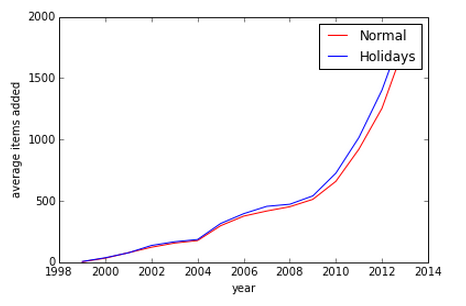
\includegraphics[width=.9\linewidth]{year.png}
  \captionof{figure}{Number of items added in normal days and holidays}
  \label{year}
\end{minipage}%
\begin{minipage}{.25\textwidth}
  \centering
  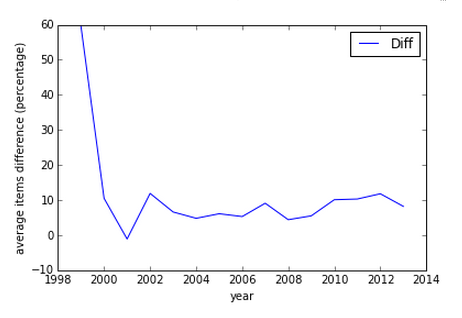
\includegraphics[width=.9\linewidth]{holiday.png}
  \captionof{figure}{Items increased in holidays}
  \label{holiday}
\end{minipage}
\end{figure}


\subsubsection{Different Holidays}
Previously we compared the shopping difference between holidays and normal days. We found that although people shop more in holidays, the increase is not that much. Our findings are against common impression that people do shop a lot in holidays, especially Thanksgiving and Christmas. We realized that it is rough to group all national holidays together to compare to normal days. We believe that holidays are also different from each other. For example people tend to shop more in Thanksgiving and Christmas. Therefore we compare different holidays in our study. Similarly, we include the last 2 days in the previous year in our analysis. There are 10 national holidays as introduced before. We again calculate the average number of items added in the nearest consecutive 5 days and compare to the average number of normal days. 

We use the data from year 1999 - 2013 and the year 2013 solely. We wish to show both the average case(from 1999-2013) and the current trend (only year 2013). We do not use data from Year 2014 because during the time of the study, the years 2014 has not been finished. Note that when computing the average item number added in normal days, we leave out all the holidays instead of simply leaving out the one that is being analyzed. The result is shown in Figure~\ref{alldiffholiday} for 1999-2013 and Figure~\ref{diffholiday} for the year 2013. In Figure~\ref{diffholiday}, The x-axis indicate the holidays accordingly (0-New Year's day, 1-Birthday of Martin Luther King, Jr, 2-Washington's Birthday, 3-Memorial Day, 4-Independence Day, 5-Labor Day, 6-Columbus day, 7-Veterans Day, 8-Thanksgiving day, 9-Christmas day).


\begin{figure}[!h]
\centering
\begin{minipage}{.25\textwidth}
  \centering
  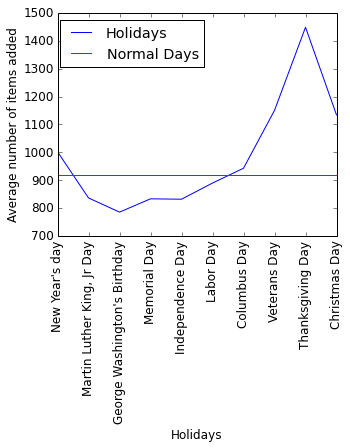
\includegraphics[width=.9\linewidth]{alldif.png}
  \captionof{figure}{Different Holidays in 1999-2014}
  \label{alldiffholiday}
\end{minipage}%
\begin{minipage}{.25\textwidth}
  \centering
  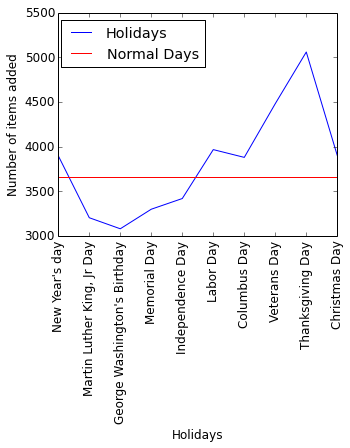
\includegraphics[width=.9\linewidth]{diff.png}
  \captionof{figure}{Different Holidays in 2014}
  \label{diffholiday}
\end{minipage}
\end{figure}


%\begin{figure}[H]
%%\minipage{0.5\textwidth}
%  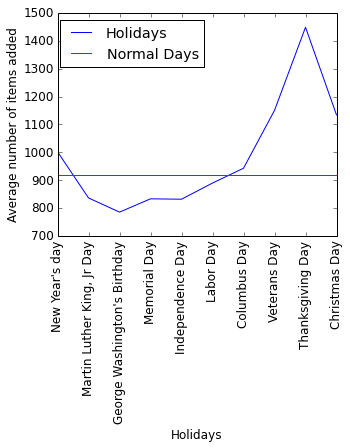
\includegraphics[width=\linewidth]{alldif.png}
%\caption{Different Holidays through 16 years}.
%\label{alldiffholiday}
%\endminipage\hfill
%\minipage{0.5\textwidth}%
%  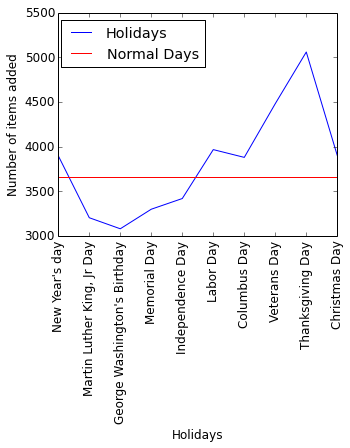
\includegraphics[width=\linewidth]{diff.png}
%\caption{Different Holidays in 2014}.
%\label{diffholiday}
%\endminipage
%\end{figure}


According to Figure~\ref{alldiffholiday} and Figure~\ref{diffholiday}, we find that holidays have huge difference between each other. In addition, we make the following observations:
\begin{enumerate}
\item The 2 figures match very well, which means that people do not tend to change their shopping behaviors at least during a short period of time. 
\item Some of the holidays are not much different from normal days (For example, Columbus Day). What is more, some of the holidays make the people less willing to add items in their wish lists. 
\item New Year's day, Veterans day, Thanksgiving, and Christmas day are 4 holidays that have quite obvious shopping increase. The result indicates that people tend to buy more stuff during the 4 holidays. The increase rate is 4.1\%, 25.2\%,72.8\%, and 30.2\% accordingly for all 15 years we analyzed. 
\item Among the 4 holidays, Thanksgiving day is the most shopping appealing holiday, which is 72.8\% higher than normal days. It is reasonable because people always get considerable discount during thanksgiving days. Christmas is the second most shopping appealing holiday because people always need to buy presents during Christmas.
\item At the first glance it is surprising that 4 holidays -- Birthday of Martin Luther King. Jr, Washington's Birthday, Memorial Day, Independence Day, and Labor day -- clearly have even less items added to user Wish Lists. The drop percentage is 10.7\%, 11.8\%, 9.0\%, 11.3\%, and 4.6\%. One possible reason is that People are more likely to be involved in other activities other than shopping during these holidays. 3 out of the 4 holidays are memorial days. Certainly these days are considered not good for shopping. 
\end{enumerate}